%======================================================================
\chapter{Control Algorithms}
\label{ch: Chapter3}
%======================================================================
This chapter discusses the three control algorithms used in the experiment.  These are linear quadratic regulator (LQR), linear quadratic gaussian (LQG), and approximate dynamic programming (ADP).
%----------------------------------------------------------------------
\section{LQR}
%----------------------------------------------------------------------
LQR is a optimal control algorithm that is used to calculate the control gain.\\%Keeping // to start new line because it looks nicer on pdf
    After creating the system model
    \begin{equation}
        \dot{x} = Ax + Bu
    \end{equation}
    use the state feedback law
    \begin{equation}
        u = -Kx
    \end{equation}
    to minimize the quadratic cost function:
    \begin{equation}
        J(u) = \int_0^\infty (x^TQx + u^TRu + 2x^TNu)dt
    \end{equation}
    Find the solution $S$ to the Riccati equation
    \begin{equation}
        A^TS+SA-(SB+N)R^{-1}(B^TS+N^T)+Q=0
    \end{equation}    
    Calculate gain, $K$
    \begin{equation}
        K=R^{-1}(B^TS+N^T)
    \end{equation}

%----------------------------------------------------------------------
\section{LQG}
%----------------------------------------------------------------------
LQG utilizes gain calculated in LQR but it adds a Kalman filter to reduce external disturbances to the system.


%----------------------------------------------------------------------
\section{ADP}
%----------------------------------------------------------------------
ADP is a reienforcement learning approach.  It utilizes the error of the state variables and feeds them into a hidden layer of neurons as shown in figure~\ref{fig:ADP_Neural_Network}.  Each of these neuron uses a quadratic activation function which is a function of error.  The result of these nodes are mutiplied by a weight which is then sent to an output node where they are summed.  This value is then used to calculate the control gain. 
\begin{figure}[!htbp]
    \centering
    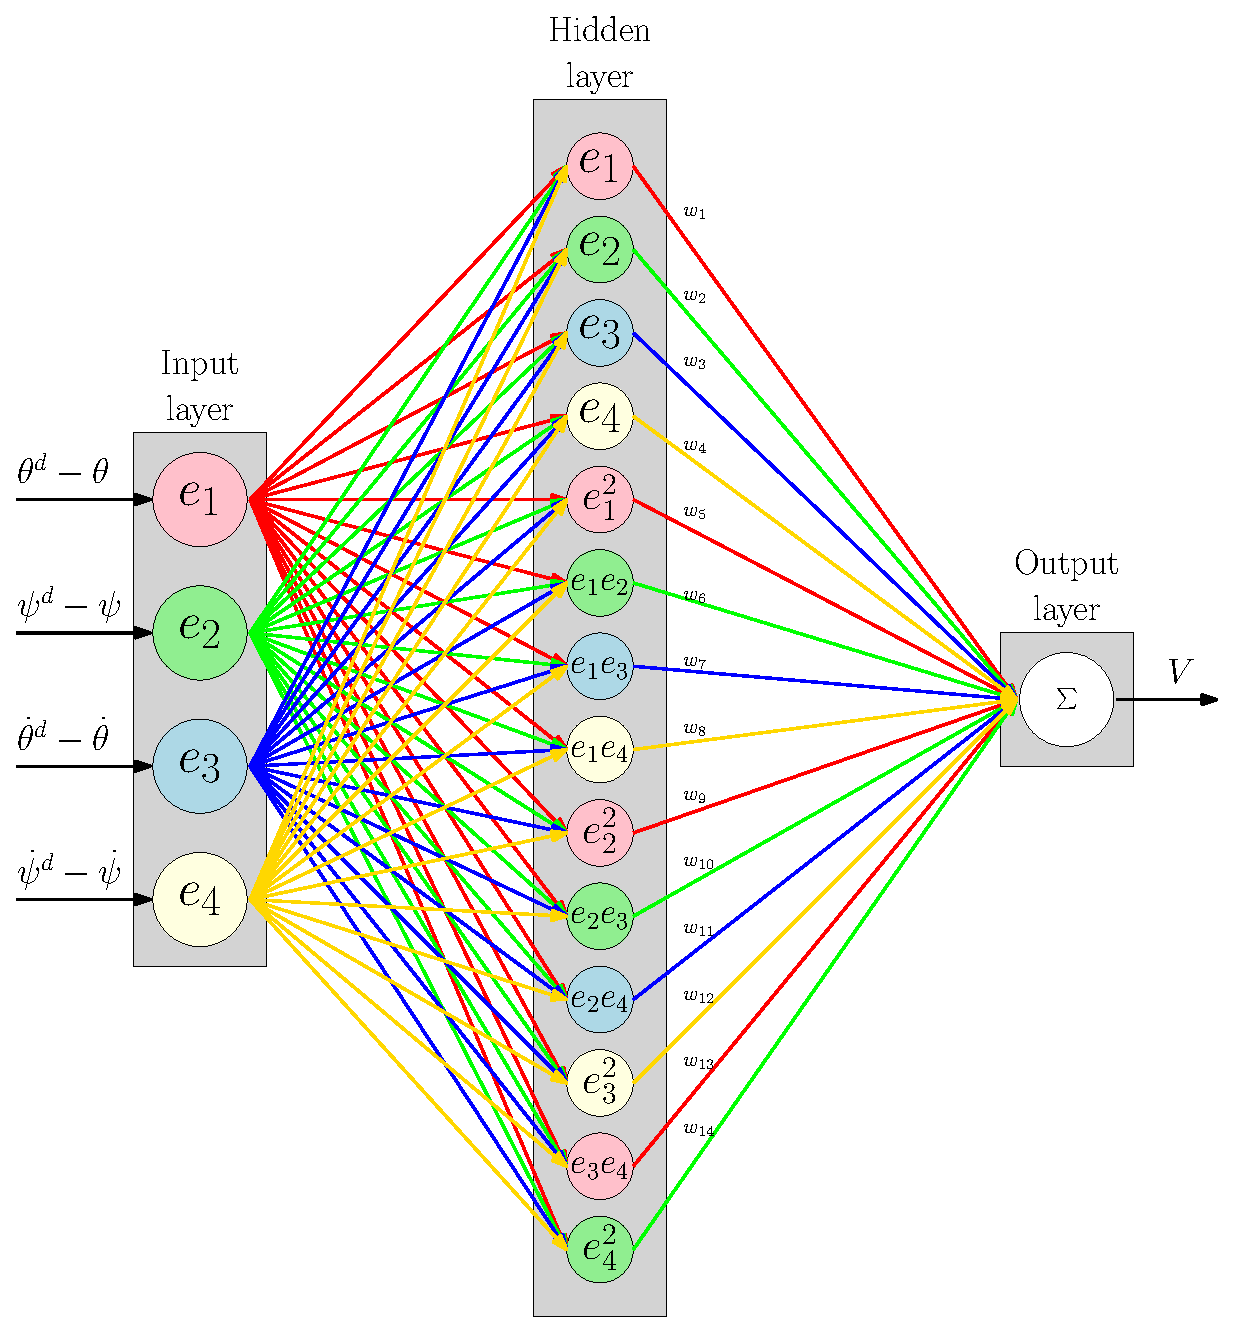
\includegraphics[width=.46\textwidth,keepaspectratio=true]{figs/ipe/ADP_Neural_Network.eps}
    \caption{Input nodes are connected to the hidden layer and then to the output layer.}
    \label{fig:ADP_Neural_Network}
\end{figure}
While the system is running, the controller is collects data every $\tau$ seconds as shown in figure~\ref{fig:ADP_Samples}.  After $T$ seconds, the data is then fed back into the neural network where the weights are updated.
\begin{figure}[!htbp]
    \centering
    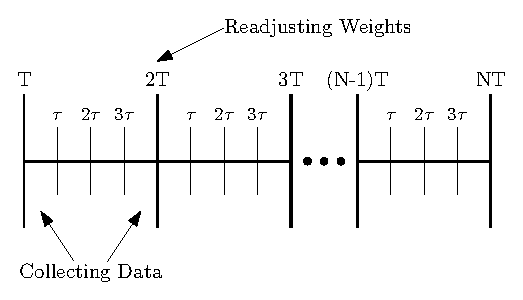
\includegraphics[width=.46\textwidth,keepaspectratio=true]{figs/ipe/ADP_Samples.eps}
    \caption{Data is collected for every $\tau$ seconds and then the weights are adjusted every $T$ seconds.}
    \label{fig:ADP_Samples}
\end{figure}

%----------------------------------------------------------------------
\section{Improvements}
Most of these algorithms are typically implemented only using proportional gain which causes steady-state error to certain input signals in some systems.  In our case, we experience steady-state error for a step input.  To reduce this, the type of the controller needs to be increased by adding an integrator.  We solve this problem by implementing a PI controller where LQR and ADP are used to find the optimal proportional and integral gain.

This is done by creating a new state varible to the system which will represent the integrated state.   As a result, the A and B will need to be augmented matrix with different dimensions.  This will also result in a different dimension of the K matrix.  The K matrix will nedd to be seperated into proportional and integral gain.

%----------------------------------------------------------------------



%%% Local Variables:
%%% mode: latex
%%% TeX-master: "../finalReport"
%%% End:
